For a thorough examination of the language, DEF has a language wiki,\cite{DEFWiki} however, a brief comparison with C is provided to show that it is, in fact, close to the machine in the same way that C is, albeit with a different syntax.  The DEF compiler is based on the Tapir branch of LLVM, that adds fork-join parallelism primitives.\cite{TAPIR,LLVM}  At present, it only runs on Linux.  The front-end is principally written in OCaml, but includes some C++.

Likewise, the \texttt{defghi} utility is written in OCaml,\cite{DEF} and is described in the Compatibility section.

Finally, the suite of microbenchmarks was developed in DEF and C with the driver in DEF.  The concurrent set and priority queue data structures selected for the suite were chosen for high performance and variety.

\subsection{Close to the Machine}

\begin{figure}[htbp!]
        \centering
        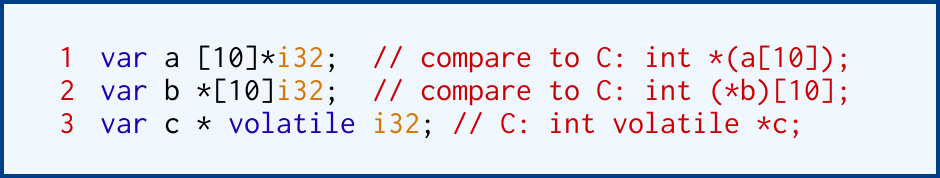
\includegraphics[scale=0.25]{gfx/types}
        \caption{Examples of variable declarations in DEF.  C allows the parentheses to be omitted in the first case, though they're provided to make precedence explicit.}
        \label{fig:types}
\end{figure}

Syntactically, DEF has some similarity to C with the most apparent difference being that scopes are denoted by keywords instead of curly braces (e.g., \texttt{if}/\texttt{then} and \texttt{fi}, \texttt{do} and \texttt{od}, etc.) allowing curly braces to be repurposed for tuples.  Native types specify a bit width, so C's \texttt{int} on most systems corresponds to DEF's \texttt{i32}.  Types are also designed to read left-to-right, so the return type in a function declaration has been moved to the right using an arrow notation similar to ML-like languages or Go.  For more complicated types, fig.~\ref{fig:types} gives an example of left-to-rightness where no parentheses are needed to distinguish an array of pointers to integers (line 1) from a pointer to an array of integers (line 2).  Volatility behaves the same as C, but the \texttt{volatile} keyword modifies only the part of the type to its right (line 3).

The expressibility is equivalent to C.  Arrays, for example, contain no metadata and can appear on the stack or on the heap.  DEF is able to commit to native integers and floating point variables of specific width, however, because architectures have largely settled on them.  C acknowledges this as of the C99 standard with types like \texttt{int32\_t} defined in the \texttt{stdint.h} header file.\cite{C99FWInts}

\begin{figure}[htbp!]
        \centering
        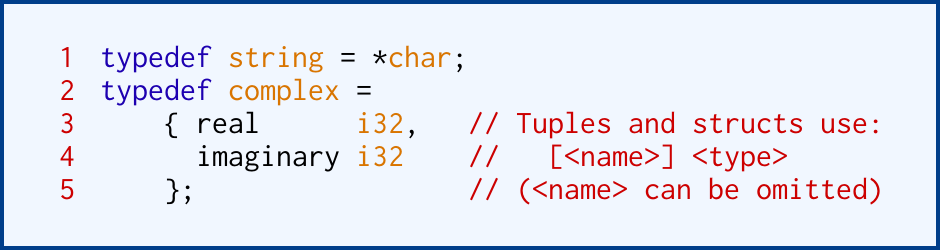
\includegraphics[scale=0.25]{gfx/typedef}
        \caption{Defining types with \texttt{typedef}.}
        \label{fig:typedef}
\end{figure}

Types are defined with the \texttt{typedef} keyword.  Figure \ref{fig:typedef} shows two examples: a C-style \texttt{string} type is defined on line 1, and a complex number struct is defined on lines 2-5.  The struct's actual definition is identical to tuple syntax, though tuples typically omit the member names.  Worthy of note is that tuples in DEF really are just anonymous structs, in keeping with the design goal of inter-operability with C.  Whereas in many languages tuples are allocated on the heap and garbage collected, in DEF they're allocated however a named struct would be in C.  Locating a struct or tuple on the heap requires explicit allocation.  Fig.~\ref{fig:window-find} provides a \texttt{window\_{}find} function declaration from the Harris lock-free linked list\cite{Harris} in Herlihy and Shavit,\cite{HSBook} as expressed in C (lines 2-6) and DEF (lines 9-10).  In both cases, the struct is returned by value on the stack.  A pointer, in both languages, would require explicit pointer syntax.

\begin{figure}[htbp!]
        \centering
        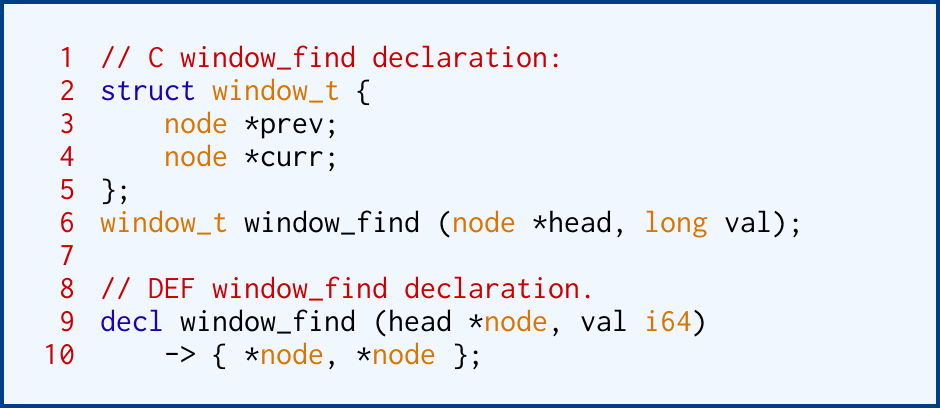
\includegraphics[scale=0.25]{gfx/window-find}
        \caption{Equivalent \texttt{window\_{}find} declarations in C and DEF.  The DEF tuple is an unnamed equivalent of C's \texttt{window\_{}t}.}
        \label{fig:window-find}
\end{figure}

Binary RMW operations with sequential consistency can be expressed by applying an \texttt{atomic} modifier to the target operation.  Fig.~\ref{fig:atomic} shows an example of \texttt{atomic} being used to add into the variable \texttt{a}.  The semantics are the same as the given C intrinsic.

\begin{figure}[htbp!]
        \centering
        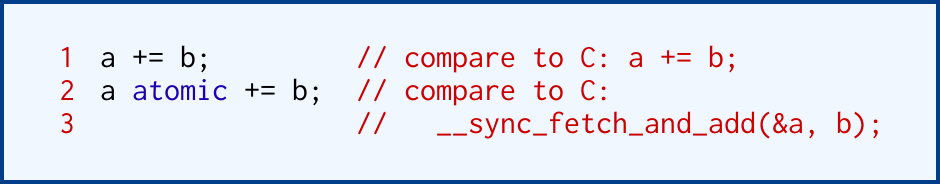
\includegraphics[scale=0.25]{gfx/atomic}
        \caption{Example of modifying a non-RMW operation to make it RMW in DEF.  The C atomic is available since C11.}
        \label{fig:atomic}
\end{figure}

Data layout is also programmer-defined.  Structs and tuple members are arranged in the order specified and aligned according to the native alignment of the underlying types.  Fig.~\ref{fig:packed} shows an example of a packed data structure in C (lines 1-2) and DEF (line 4).  Packed structs and tuples have the minimum addressable alignment, as do their members, and are packed as tightly as the architecture permits.  In C, this is accomplished through compiler-specific attributes, but the existence of these attributes is widely supported.

\begin{figure}[htbp!]
        \centering
        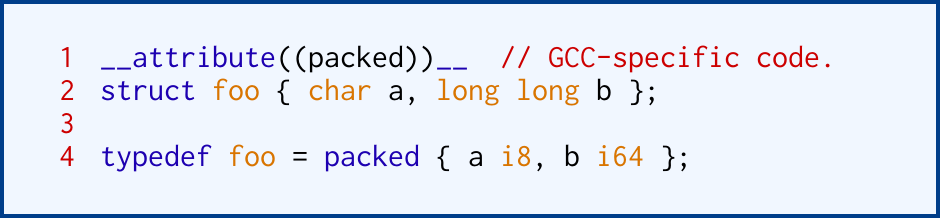
\includegraphics[scale=0.25]{gfx/packed}
        \caption{\texttt{packed} in front of a tuple specifies alignment of the members.}
        \label{fig:packed}
\end{figure}

Despite the difference in syntax, DEF exhibits the same kind of expressibility as C in data layout and instruction generation.  There aren't unexpected hidden costs in operations or types, allowing a programmer to tune DEF code for performance in the same way as one would do for C.

\subsection{Modularity}

As above, modularity is decided by the profile presented to users of a library.  In a concurrent data structure, what does a programmer need to know about pointers returned from thus-and-such a function call?  What are the restrictions?

DEF has no native allocator.  Allocating memory with \texttt{new} and deallocating it with \texttt{delete}, use \texttt{malloc} and \texttt{free}, respectively.  Since DEF's memory reclamation system is implemented using Forkscan, they implicitly use Forkscan's \texttt{malloc} and \texttt{free} wrappers, but the overhead of this indirection is undetectable in trials.  Independent of implementation, memory allocated with \texttt{new} is untracked.  Memory can be passed freely between DEF and C, and a pointer acquired in C through \texttt{malloc} can be deleted in DEF, and one acquired in DEF through \texttt{new} can be freed in C.

Moreover, \texttt{new} and \texttt{delete}, as applied to non-shared memory, are conveniences-only.  Mixing allocators or interfacing with a language with hooks to an external garbage collector is as trivial (or as complex) in DEF as it is in C because all memory is treated in exactly the same way.

The exception to this is in the use of \texttt{retire} to flag a pointer for tracking.  \texttt{retire} cannot be applied arbitrarily to pointers since there is no way to determine origin.  DEF assumes that a retired node was allocated with the same allocator used by \texttt{new}.  Implementation-wise, Forkscan requires knowledge of the \texttt{free} and \texttt{malloc\_{}usable\_{}size} corresponding to the \texttt{malloc} that was used to acquire the memory.  More broadly, it's hard to see how any implementation could call the correct \texttt{free} on a retired node unless it corresponded to the known \texttt{malloc} for the same reason.  This is not especially burdensome to programmers since mixing allocators is typically frowned upon as it makes code needlessly complex.

A final restriction on \texttt{retire} is that it may only be called on a pointer, once.  If multiple threads retire the same memory, the behavior is undefined.  In practice, it acts like a double-free because the reclamation system may perform a double-free.  A good usage model is the thread that successfully removes a node from the concurrent data structure is the one that should retire it.  This makes its use intuitive because code looks like the familiar serial model where \texttt{retire} is replaced by \texttt{delete}.

Forkscan was modified to accommodate these semantics.  When Forkscan completes a memory sweep, it creates a pool of pointers known to have no outstanding references in the user program.  As originally implemented, every call to \texttt{forkscan\_{}malloc} first frees a few of these pointers.  But this creates a dependency on \texttt{forkscan\_{}malloc}.  If a C module na\"ively, repeatedly calls \texttt{malloc} (as opposed to \texttt{forkscan\_{}malloc}), even from the correct allocator, and gives the memory to a DEF module that retires it, unless the DEF module is also independently allocating its own memory with \texttt{new}, none of the retired memory will ever be reused.  This is a practical leak.  The modification moved the burden from \texttt{forkscan\_{}malloc} to \texttt{forkscan\_retire}, eliminating the dependency.

This produced no discernable difference in performance.  The reasoning for the original design was that freeing memory and then immediately allocating would likely return a pointer to memory that was already in the cache.  High performance allocators tend to have this property.  Changing the location of the burden didn't affect performance because, even if \texttt{malloc} wasn't called immediately after \texttt{free}, the delay between retiring and allocating memory wasn't very great, and the allocated memory was probably still in the cache.  Since some of the concurrent data structures tested were among the most high-performance known, we reason that the change has little or no effect on performance.  Even in a producer/consumer application, where \texttt{malloc} is being called with high frequency such that whether memory is in cache has a measurable impact on performance, the likelihood is that the producer is getting memory from the cache in a high performance allocator, anyway.

\subsection{Compatibility}

C++ is the gold-standard for interfacing with C.  As mentioned above, C header files can be included directly into C++ files, and C++ functions can be declared with C linkage.  Features like templates, classes, and member functions of structs can't be exported to C, but anything C-like can be.  Given DEF's syntactic differences, even for features common with C, sharing DEF interface (\texttt{.defi}) files directly with C is impossible.  However, most of the function-level features have a one-to-one correspondence with C.  Therefore, the compiler is accompanied by a utility, \texttt{defghi}, for generating headers and interface files from DEF source files.

Generating headers and interface files is assisted by DEF's explicit approach to module interfaces.  A subtle distinction from C is that DEF types, functions, and globally-scoped variables are local to the module in which they appear, by default.  C's default is external visibility, and local symbols must be marked \texttt{static} by the programmer.  In contrast, DEF's default visibility is local and requires programmers to mark symbols with \texttt{export} in order to make them available to other modules.

Generating header files from \texttt{defghi} is simple since the differences in declarations are syntactic.  Any type, global variable, or function marked \texttt{export} has its declaration unparsed into C and pretty-printed into the target header.

\begin{figure}[htbp!]
        \centering
        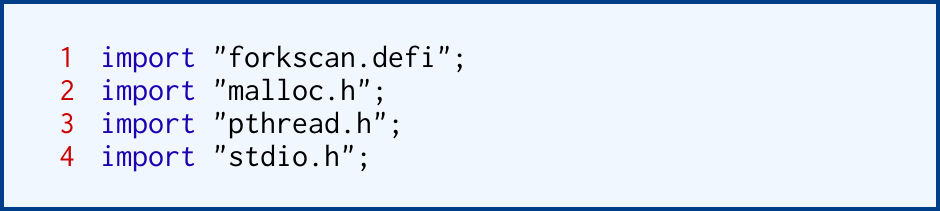
\includegraphics[scale=0.25]{gfx/import}
        \caption{Snippet of code from the actual benchmark importing DEF interface files and C header files.}
        \label{fig:import}
\end{figure}

The other direction, importing C definitions into DEF (fig.~\ref{fig:import}), involves recognizing headers by filename extension and passing them through a C parser.  Clang, the LLVM C compiler, collects all type definitions and function and global variable declarations, and DEF converts them into its own internal representation.  Therefore, DEF can import C headers directly as if they were native DEF.

There are two limitations to this: DEF can't import actual C functions (as opposed to function declarations), and C macros aren't resolved except where they appear in a header file itself.  In the first case, functions in header files are a planned feature that was deprioritized since they're uncommon in the C standard library, and it was reasoned that high performance programmers often do intermodule optimization, negating the value of putting them in headers.  In the second case, DEF does not yet have macros of its own, and a na\"ive implementation of incorporating C macros might conflict with a well-designed DEF macro language.  Since C macros are simple text-substitution, integration into a language with a different syntax is another problem, altogether.

Even with the current limitations, however, DEF is able to import the C standard libraries, use their types, call their functions, and access their global variables.

\subsection{Concurrent Data Structures}


The are two classes of data-structures chosen for our comparison, sets and priority queues each with their own benchmark driver. In the set benchmark, items are randomly added and removed at a specified update rate. For the priority queues either a random element is added or the minimum element is removed.

\paragraph{Skip List} A fixed-height lock-free skip list was included as a well-known probabilistic concurrent data structure.  Each node contains one value, and the nodes are arranged in a list with a set of one or more forward pointers.  Each forward pointer points to the next node with at least that height, and the height of all nodes averages two.  Operations take logarithmic time, as they would in a binary tree, but tend to have better cache behavior. A node is retired by the thread that swings the lowest height pointer during the removal of a node; a one-line change to the algorithm as described in Herlihy-Shavit.\cite{HSBook}

\paragraph{Hash Table} The lock-free separate chaining hash table performed favorably in Michael's tests.\cite{HashTables} Each bucket in the hash table contains a lock-free linked list by Harris.\cite{Harris} The list at each bucket is sorted and allows for early search termination. Like the Harris list a window of nodes is kept during the \texttt{find} procedure and used in insertion and removal. Nodes in the list are removed by marking the current node's next pointer, effectively locking that node. This stops another node from being inserted in front of the current node marked for deletion. Finally the removing thread swings the previous node's next pointer to the next pointer of the current node being removed, splicing the current node out of the list. Other threads that see a marked next pointer help remove the marked node from the list, making the remove operations cooperative and lock-free. During out experiments the average list length at each bucket was kept at 36 nodes.

\paragraph{Binary Tree} The fast concurrent lock-free binary search tree by Natarajan and Mittal is a recent concurrent data structure that operates by marking edges rather than nodes.\cite{LFBinaryTree} The algorithm is relative simple and fast due to the lack of any rebalancing algorithm. Rebalancing algorithms are a source of contention as some require a potentially global data-structure reorganisation. The data-structure is an external binary tree, meaning the values of the set are stored in the leaf nodes rather than throughout the tree. The internal nodes are only for routing and serve no other purpose. The work-horse of the data-structure is the \texttt{seek} method. Like the Harris linked list, \texttt{seek} constructs a window of the tree while searching. \texttt{Seek} will exclude nodes that have been marked for deletion as those nodes cannot be valid ancestors for replacement when removing. The tree contains a fixed amount of nodes which are never removed so that there will always be a valid node family tree. Removing a node is a two stage process and requires two bits. The two bits represent \textit{flagging} and \textit{tagging} of an edge. To remove a node first the thread first marks the parent's edge to the node, this mark is a flagging operation. The second marking takes place in the \texttt{cleanup} method, \texttt{cleanup} is run when a modifying operation sees a \textit{flagged} edge to a node. The second marking is done on the sibling node of the node to be removed, this marking is called \textit{tagging}. Once both edges (of the parent) have been marked no other modifying operation can occur and now the parent and the node to be removed can be unlinked. Like deletion, retiring is a two stage process. The thread that initially injects the deletion, via \textit{flagging} an edge, retires the leaf node. Later the thread that replaces the successor in \texttt{cleanup} with the sibling of the to be deleted node retires the successor node.

% \paragraph{Shavit Lotan Queue} This was included as an example of a skip list-based priority queue. \cite{ShavitLotanQueue} The Shavit Lotan Queue is a lock-free priority queue data-structure where the \texttt{pop-min} method traverses the lowest height/level of the skip list. Since the skip list is a series of sorted linked lists, with the lowest height/level containing all values, threads can remove the top items from the list which have the highest priority. Deletion is done logically, using the atomic swap (or similar CAS) to mark a node as deleted and then physically removing that node at that point or sometime after. Timestamps can be added to each node in order to make the list linearisable \cite{Linearizability}, otherwise the structure is quiescently consistent (cite). As in the skip list, the node is retired by the thread that swings its lowest height pointer.

\paragraph{Lind{\'e}n Jonsson Queue} This was included as an example of a skip list-based priority queue. \cite{LindenPriority} The Lind{\'e}n Jonsson Queue is a lock-free priority queue data-structure where the \texttt{pop-min} method traverses the lowest height/level of the skip list. Since the skip list is a series of sorted linked lists, with the lowest height/level containing all values, threads can remove the top items from the list which have the highest priority. Deletion is done logically, using the atomic swap (or similar CAS) to mark a node as deleted with physical deletion delayed until some point after. Physical deletion is done in batches and is quite efficient, the size of the batch is specified ahead of time. The thread which performs physical deletion is responsible for retiring the nodes.

\paragraph{SprayList} Finally, the benchmark includes a SprayList priority queue.\cite{SprayList} The SprayList is based on a skip list, but the node to remove is selected probabilistically from near the beginning to reduce contention. This probabilistic walk is referred to as the \textit{spray} and is paramount to reducing contention from threads. The SprayList is a relaxed concurrent data-structure whereby \texttt{pop-min} will remove from a range of top items in the list. The range and other parameters of the \textit{spray} are initialised by the number of expected threads (concurrency) acting on the queue. Because nodes closer to the beginning are less likely to be \textit{landed-on} after the \textit{spray}, padding nodes are added to the beginning of the list. Once the SprayList \textit{sprays} it will continue in the same fashion as the Lind{\'e}n Jonsson Queue and traverse the lowest level of the list until a deleted node is found. Under high contention the SprayList can scale significantly better than traditional concurrent priority queues, but it can be very sensitive to the choice of spray parameters. As in the skip list, the node is retired by the thread that swings its lowest height pointer.

